\section{Parameter estimation results}
\label{sec:ERA_results}
Since everything in the simulator is inside Simulink, it is not too hard to get noise-free measurements, which means no experiments had to be repeated to suppress noise or disturbances. A step-response seemed to work better with the simulator than an impulse-response,so that was used instead. The diagonal of $\Sigma$ after a singular value decomposition can be used to say something about how much adding additional states in a model will help in lowering the estimation error. 


\begin{figure}
    \centering
    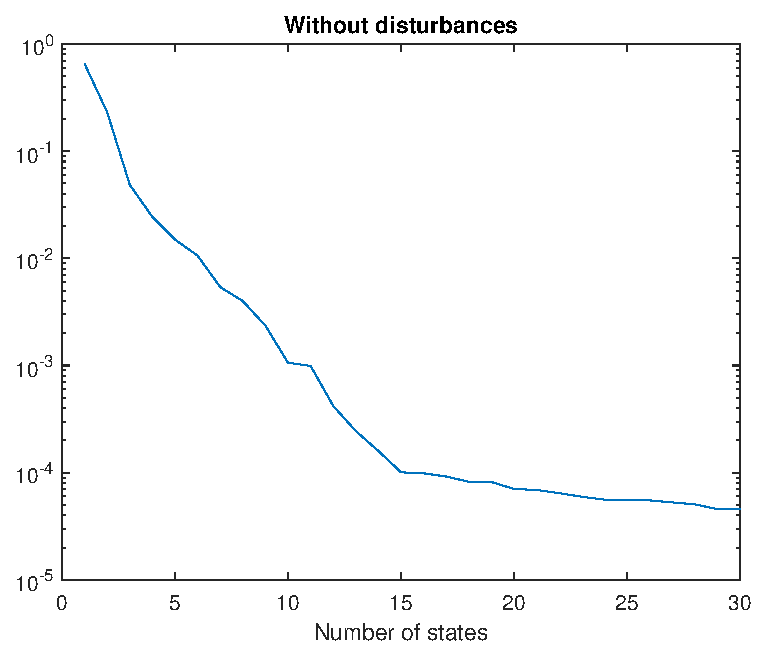
\includegraphics[width=\textwidth]{img/Fig_dump/Sigmas_without_disturbances.eps}
    \caption{$\frac{\Sigma_{i,i}}{sum_{j=1}^{N}(\Sigma_{j,j})}$ from the SVD $U\Sigma V^* = H_1$}
    \label{fig:ERA_state_contributions}
\end{figure}
\todo[inline]{I left off correcting this section @@@. Add the proper figures}
\noindent
From the plot in figure \ref{fig:ERA_state_contributions}, it can be seen that the diagonal elements of $\Sigma$ decrease quite rapidly. Using too many parameters will often cause a mode to be overfitted, which can lead to problems. As a result, models of order 5,7, 10, 12 and 15 were tested. To validate the estimated models, they were plotted against the original step-response. 


\noindent
As can be seen in figure \ref{fig:unscaled_system_approx}, even the 10th order models struggles with estimating certain outputs. This is because the inputs and outputs have not been scaled properly, so the total error will go down significantly more if the error in the $HHV$ is reduced a little, than if the error in $Y_{O2}$ is eliminated. The solution to this is to scale the inputs and outputs somewhat. One formulation for the goal of the scaling can be set is to make as many input-output relations have an amplitude of 1 for some norm (max, $\mathcal{L}_2$, etc.). There is probably a method to finding the optimal solution to this problem, but for the sake of simplicity, it is also possible to alternate between scaling the inputs and the outputs, such that the largest norms, are equal to 1. The exact method is not that important, as long as the HHV or $v_{grate}$ does not dominate the estimation. 

\begin{figure}
    \centering
    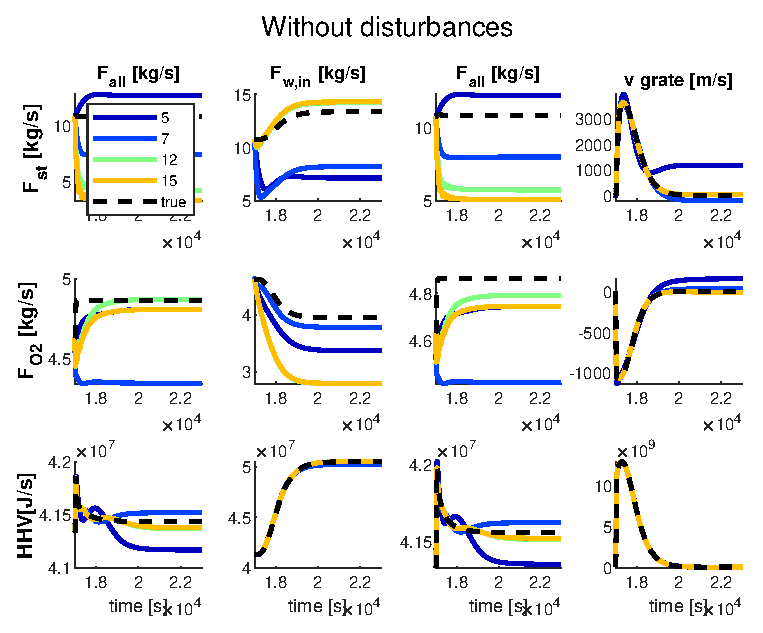
\includegraphics[width=1\textwidth]{img/Fig_dump/Unscaled_ERA_step_approx_without_disturbance_inputs.eps}
    \caption{Approximation from unscaled measurements. The lack of scaling causes an over-fixation on $\hat{HHV}$ and $v_{\text{grate}}$}
    \label{fig:unscaled_system_approx}
\end{figure}



\noindent
After using ERA to estimate the system, it can be scaled back with the same vectors. The result, as seen in figure \ref{fig:proper_system_approx}. The resulting approximated system has a far lower relative error. This scaling is necessary for creating an accurate low-order model that can be used for controlling all outputs of the plant, not just the estimated HHV-value.

\begin{figure}
    \centering
    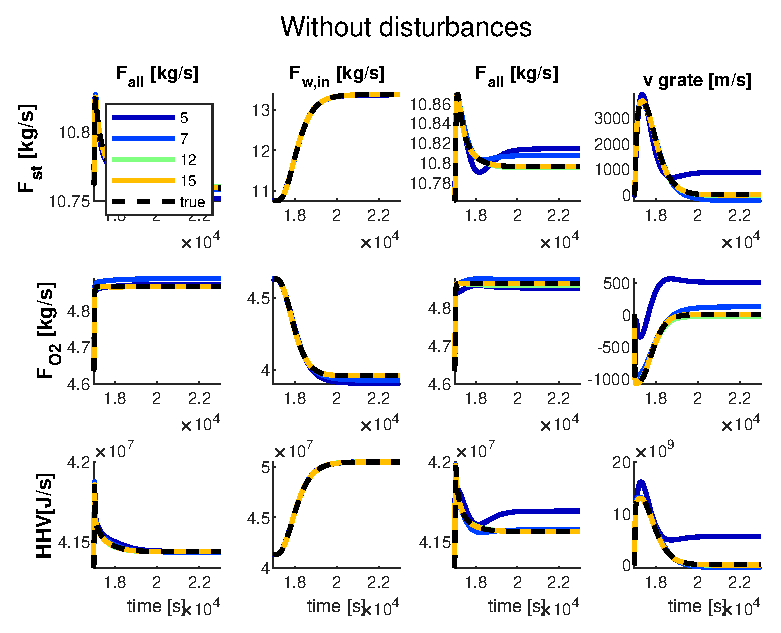
\includegraphics[width=\textwidth]{img/Fig_dump/ERA_step_approx_without_disturbance_inputs.eps}
    \caption{Approximation from scaled measurements. The relative error is now much smaller}
    \label{fig:proper_system_approx}
\end{figure}

\subsection{Choosing a model order}
Picking a model order can be somewhat difficult. From what can be seen in figure \ref{fig:proper_system_approx}. All estimates struggle with matching some of the outputs. Most importantly is the relation between the input air and steam production. Using a model with 7 states might look sufficient at first, but later experiments who that  a model order of 12 was found to greatly outperform it when attempting to control the plant. The reason for why the model has to be so precise is most likely because the controller can get an immediate increase in steam production by increasing $F_{aI}$ while decreasing  $F_{aII}$. If the controller uses this method to suppress immediate changes in steam-production, then this part of the model has to be as precise as possible. 

\subsection{Expanding the model with disturbances}
\todo[inline]{}
Additional experiments were also performed in an attempt to estimate a model for both process disturbances and normal inputs. Figure \ref{fig:ERA_distrubance_state_contributions} shows how much each each state contributes to the new approximation. Figure \ref{fig:ERA_state_contributions} and \ref{fig:ERA_distrubance_state_contributions} are remarkably similar, but the model without disturbances decreases faster in the beginning, which is the reason for why a simpler model can be chosen. 


\begin{figure}%#TODO Add the sigma plot
    \centering
    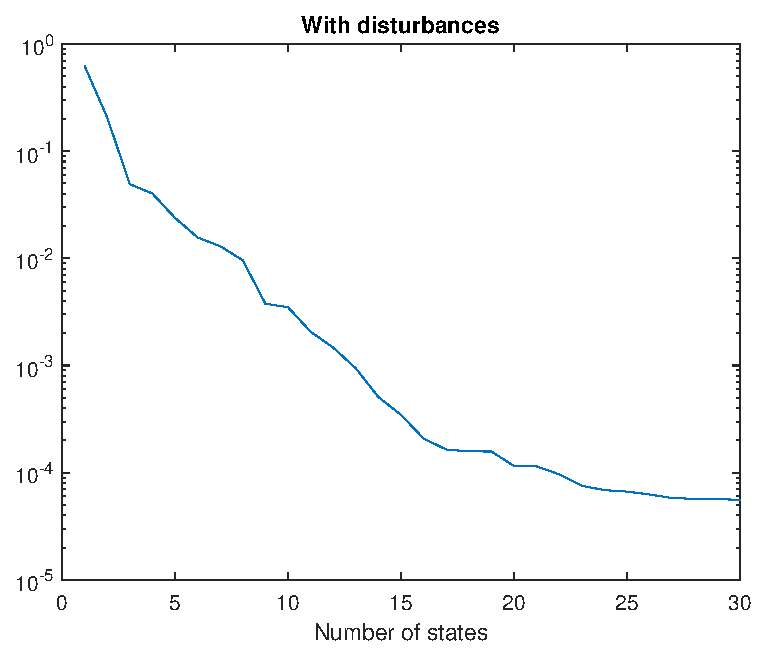
\includegraphics[width=\textwidth]{img/Fig_dump/Sigmas_with_disturbances.eps}
    \caption{$\frac{\Sigma_{i,i}}{sum_{j=1}^{N}(\Sigma_{j,j})}$ from the SVD $U\Sigma V^* = H_1$}
    \label{fig:ERA_distrubance_state_contributions}
\end{figure}



\noindent
Just like in the previous model, the inputs and outputs have to be scaled to get a decent model. Additionally, the extra inputs representing the measurements require a more complex model if everything is to be modelled somewhat properly. As a result, a model of order 15 is used instead of a model of order 12. 

\begin{figure}
    \centering
    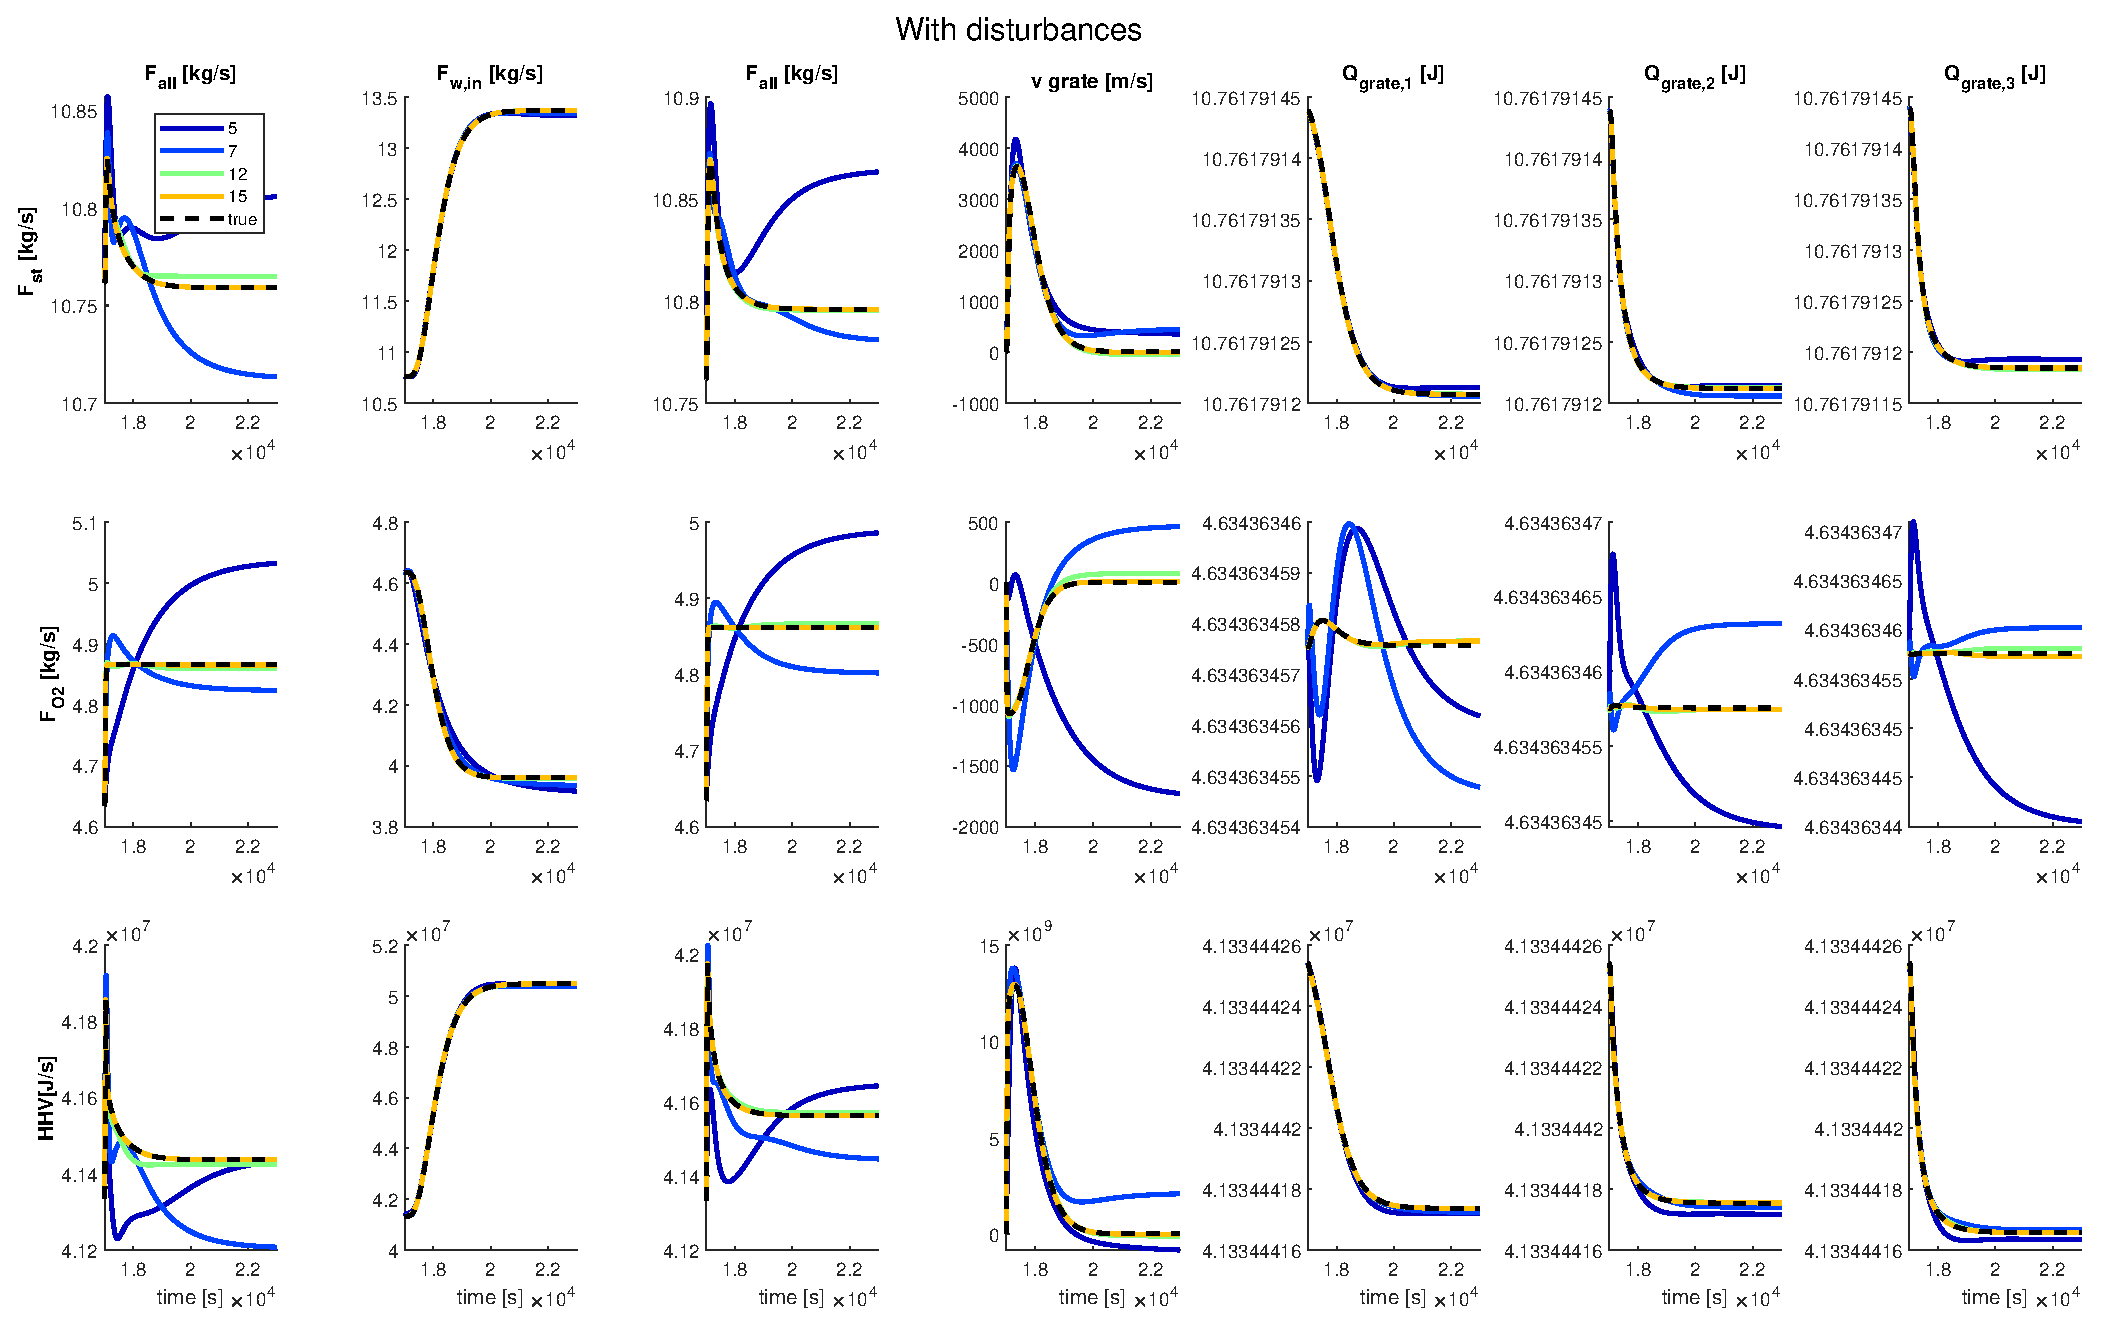
\includegraphics[width=\textwidth]{img/Fig_dump/ERA_step_approx_with_disturbance_inputs.eps}
    \caption{Model that also shows the dynamics of disturbances}
    \label{fig:disturbance_proper_system_approx}
\end{figure}

\noindent 
The estimated response reinforces the notion that Q_grate does not affect $F_{O2}$ very much. This is also the reason as for why the model seems to struggle more with those outputs than most of the other input-output relationships. 

